I now use the industry-level data to demonstrate why the absence of a reallocation effect in previous studies is puzzling. The aggregate labour share in year $t$, $\lambda_{t}$, can be written as the weighted sum of sectoral labour shares
\begin{equation}
\begin{split}
    \lambda_{t} &= \sum_{i=1}^{N}\omega_{it}\lambda_{it}
\end{split}
\label{eqn:weighted_ls_second}
\end{equation}
in which $\omega_{it}$ denote a sector's value-added-to-GDP weight in year $t$, and $\lambda_{it}$ is sector $i$'s labour share of value-added.

\noindent First, towards which sectors does the economy reallocate since 1987? The left panel in figure \ref{fig:GS} shows the share of value-added shifted towards service-producing industries since 1987, which is already well documented in the literature (e.g. \citet{herrendorfTwoPerspectivesPreferences2013, bridgmanLaborShareMarkups2023}). Second, how do labour share levels and trends differ between growing and shrinking sectors? The right panel shows the average labour share in services sectors is higher and declines slower than in goods sectors. Goods-producing industries see a much sharper drop in their average labour share from 1987 onwards. All else equal, the reallocation of value-added towards higher labour share sectors in services should partially offset the decline in the labour share. Indeed, in the right panel of figure \ref{fig:GS}, the fall in the aggregate labour share is muted relative to the larger decline in the average labour share in goods-producing sectors.


\begin{figure}[h]
  \centering
    \caption{\normalsize Value-added and average labour shares of goods and services.}
  \subfloat{\label{fig:b}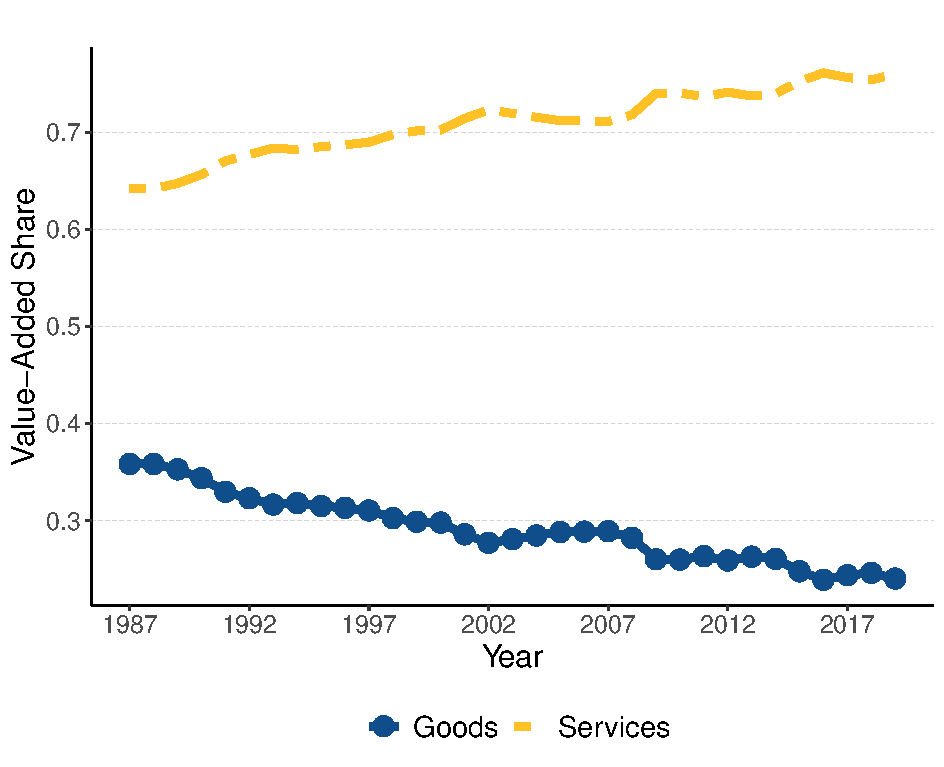
\includegraphics[width=.45\linewidth]{Puzzle/omega_GS.pdf}}
  \subfloat{\label{fig:c}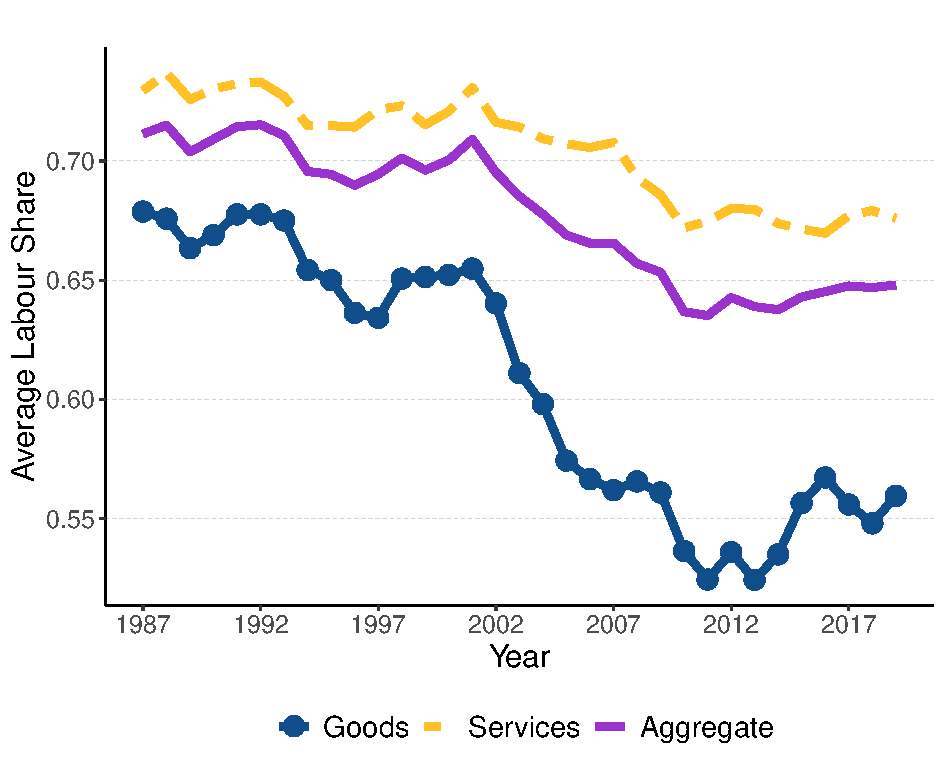
\includegraphics[width=.45\linewidth]{Puzzle/lambda_GS.pdf}}\vfill

    \label{fig:GS}

\begin{minipage}{\linewidth}
    \caption*{\textit{Notes}: The left panel shows the value-added-to-GDP share of goods and service sectors. The right panel shows the average labour share within goods and service sectors. \\
    \textit{Source}: BEA-BLS integrated industry-level production account and author's calculations.}
\end{minipage}
\end{figure}


Third, I conduct a simple counterfactual exercise in which I fix sectoral labour shares $\lambda_{it}$ at their 1987 values, allowing only the weights $\omega_{it}$ to change. The counterfactual labour share is given by
\begin{equation}
    \lambda_{t}^{\text{counterfactual}} = \sum_{i=1}^{N}\omega_{it}\lambda_{i1987}.
\label{eqn:counterfactual_ls}
\end{equation}
Figure \ref{fig:counterfactual_index} shows the counterfactual path of each labour share definition, all indexed to the 1987 aggregate labour share. For all four definitions, albeit to different extents, the counterfactual labour share is higher than the actual path. These counterfactuals suggest the labour share would have risen since 1987 if only sectoral weights (reallocation) had changed since then. Why is the positive reallocation effect missing from decompositions used in previous studies? To answer the question, in the next section I describe the the decomposition framework I apply to the industry data. 


\begin{figure}[h]
    \centering
    \caption{\normalsize Counterfactual labour shares holding sectoral labour shares fixed}
    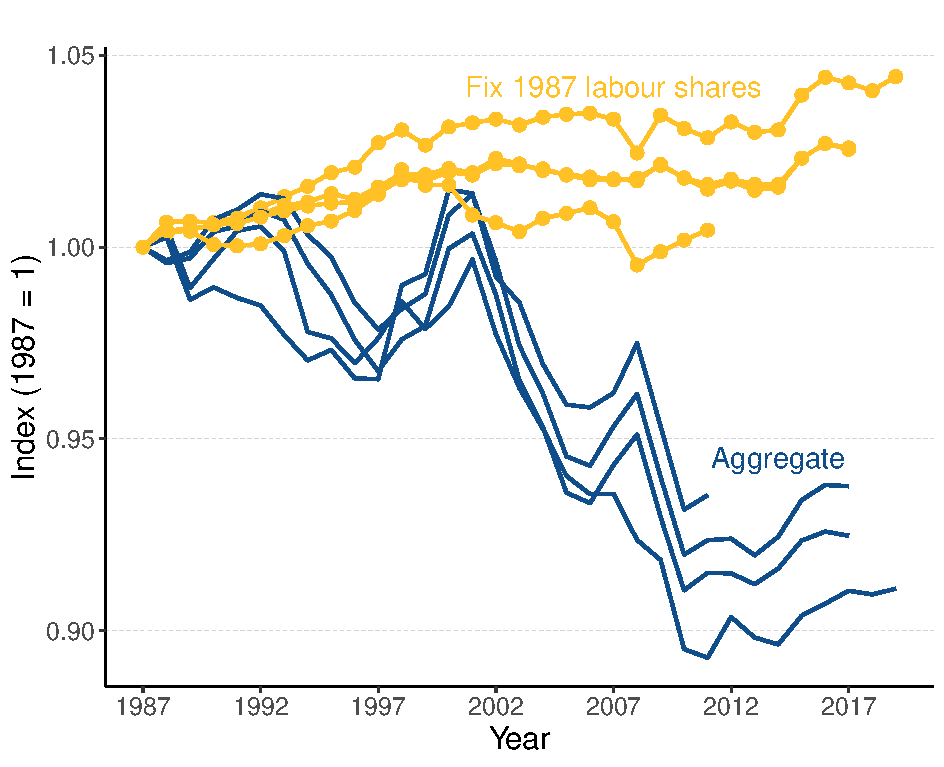
\includegraphics[width=10cm]{Puzzle/counterfactual_graph_index.pdf}

    \label{fig:counterfactual_index}

\begin{minipage}{\linewidth}
    \caption*{\textit{Notes}: The four lines sloping downward represent the path of the aggregate labour share for the four methods I use to impute self-employed labour income. The four lines sloping upward show the counterfactual paths of the aggregate labour share had sectoral labour shares stayed fixed at their 1987 values: $\lambda_{t}^{\text{counterfactual}} = \sum_{i=1}^{N}\omega_{it}\lambda_{i,1987}$. All lines are indexed to the respective 1987 labour share. \\
    \textit{Source}: Bureau of Economic Analysis (BEA), Bureau of Labour Statistics (BLS), and author's calculations.}
\end{minipage}
\end{figure}




